\chapter{Introduction}

\justifying
\section{Background}

     Artificial satellites are foundational components of modern society. Satellites have played a huge role in communication, navigation, scientific research, military surveillance and the study of the solar system and beyond. 
     
     Artificial satellites are launched into space using rockets and are placed in orbit around the Earth or other celestial bodies using thrusters. Once in orbit, they remain in space and continuously circle around the Earth, following a specific path called an orbit.
     
     There are two main types of orbits for artificial satellites: geostationary orbit and low Earth orbit. Geostationary orbit is a circular orbit located at an altitude of approximately 36,000 kilometres above the Earth's equator. Satellites in this orbit appear to be stationary relative to a fixed point on Earth, making them ideal for communication and navigation purposes. Low Earth orbit, on the other hand, is an orbit located at an altitude of up to approximately 2,000 kilometres above the Earth's surface. Satellites in this orbit circle the Earth more frequently and are used for scientific research, remote sensing, and military surveillance.
     
     Artificial satellites are powered by solar panels that convert sunlight into electricity, which is used to operate the satellite's systems and instruments. They are also equipped with communication antennas that enable them to transmit and receive signals from Earth or other satellites.
     
%      The first artificial satellite, Sputnik, was launched in 1957. The launch of the first
% meteorological satellite, TIROS-1, in 1960 was followed by the U.S. The first Earth-observing satellite for land-based applications was Landsat-1, which was launched in 1972. Since then many more Earth-observing satellites have been put into orbit.  Overall, artificial satellites have revolutionized our ability to communicate, navigate, observe, and study our planet and the universe beyond. They have become an essential part of modern life, and their applications are only expected to increase in the future.
\\

% The whole process of designing, building, and launching a satellite-flown remote sensing system is a very lengthy and costly process. The main driving force behind the enormously costly development
% of space technology has been the military, where cost is not usually a problem. With the relaxation on restrictions for ownership and operation of Earth-observing satellites it is now possible for anyone to build and launch satellites.
\\

For more than a decade, CubeSats, or small satellites, have paved the way to
low-Earth orbit for commercial companies, educational institutions, and non-profit
organizations. These small satellites offer opportunities to conduct scientific
investigations and technology demonstrations in space in such a way that is
cost-effective, timely and relatively easy to accomplish. Due to their small size, CubeSats can be launched on smaller rockets or piggybacked on larger missions, allowing for more frequent and flexible deployment opportunities. The small size of CubeSats allows for faster development and testing of new technologies, which can be later applied to larger satellites or space missions.\\


A CubeSat is a class of miniaturized satellite based around a form factor consisting
of 10 cm cubes. CubeSats have a mass of no more than 2 kg per unit, and often use
commercial off-the-shelf (COTS) components for their electronics and structure.
CubeSats are put into orbit by deployers on the International Space Station, or
launched as secondary payloads on a launch vehicle. As of August 2021, more than
1,600 CubeSats have been launched.
\\

CubeSat missions benefit Earth in varying ways. From Earth imaging satellites that
help meteorologists to predict storm strengths and direction, to satellites that focus
on technology demonstrations to help define what materials and processes yield the
most useful resources and function best in a microgravity environment, the variety
of science enabled by CubeSats results in diverse benefits and opportunities for
discovery.\\

Electrical power systems (EPS) are an essential component of CubeSats as they have a limited power budget and often require a reliable source of power to operate their payloads and subsystems. There are several ways to design an EPS for a CubeSat, and the choice depends on the mission requirements and the available resources.
The most common EPS design for CubeSats is based on solar panels, which convert sunlight into electrical energy. 

%These solar panels can be mounted on the CubeSat's surface and can use either single-junction or multi-junction solar cells. Single-junction solar cells are simple and inexpensive, while multi-junction cells offer higher efficiency but are more complex and costly.

The solar panels are typically connected to a power management and distribution unit (PMDU), which regulates the voltage and current of the incoming power and distributes it to the various subsystems and payloads. The PMDU also includes a battery that stores excess power generated by the solar panels and provides power during eclipses or when the solar panels are not receiving enough sunlight.

The EPS also includes other components such as a power switch, a fuse, and a battery charge controller. The power switch is used to turn on or off the power to the subsystems and payloads, while the fuse protects against over-current and short circuits. The battery charge controller manages the charging and discharging of the battery, ensuring that it is not overcharged or over-discharged.

The design of the EPS depends on the specific mission requirements and the available resources, and CubeSat developers must carefully balance the power budget to ensure that the CubeSat can operate reliably and efficiently throughout its mission.

\section{Objective}
%To design and implement a fully autonomous power generation, storage and distribution
%system for a CubeSat
The aim of this project is to determine requirements for a typical CubeSat Electrical Power System (EPS) and develop a working prototype of the EPS for a CubeSat.
\\ \\
  This EPS will be used as the prototype for the BARTOSAT cubeSat developed by the students of GEC, Barton Hill as a part of the Satellite Research Center of the college. The prototype will then go through various iterations, improving the design to meet all the requirements of other subsystems which are currently under development and also to make it fully capable to work in the space environment.\\

\subsection{The Satellite Research Center, GECB}
\justifying
  The Satellite Research Center of Government Engineering College, Barton Hill, is a facility dedicated to conducting research in the field of satellite technology and to help students get an exposure to space technologies in general. As a part of this, a student project was initiated, aimed at developing a 1U CubeSat named ‘Bartosat’, which will be designed to carry a LoRa module as the payload. 
 \\ \\
   Every phase of designing, building and testing of the CubeSat has been carried out by different student teams from various departments. The payload will test the possibilities of space-to-ground communication using LoRa technology, which can lead to low cost, low-power space communication.
 \\

\section{Literature Review}
\justifying
The EPS is a critical component of a CubeSat as it powers all the subsystems in the satellite. There are different EPS architectures of based on DC bus regulation and interface of PV panels [1].
\\ \\
The main challenge for the development of CubeSats is to fit all the necessary equipment within the standard frame size while meeting the weight constraints. The EPS design is crucial for the successful CubeSats mission, which needs to consider several factors such as mission duration, orbit altitude, inclination angle, size of PV panels and its arrangement, load profile, volume and weight limits, radiation effects, overall efficiency, simplicity of control, component count, flexibility in battery configuration, reliability, and fault-tolerant capability. 
\\ \\
One of the important steps in EPS design is the selection of most suitable EPS architecture. The different types of CubeSat EPS architectures are shown in Figure. 
\\ \\
\begin{figure}[h]
	\centering
	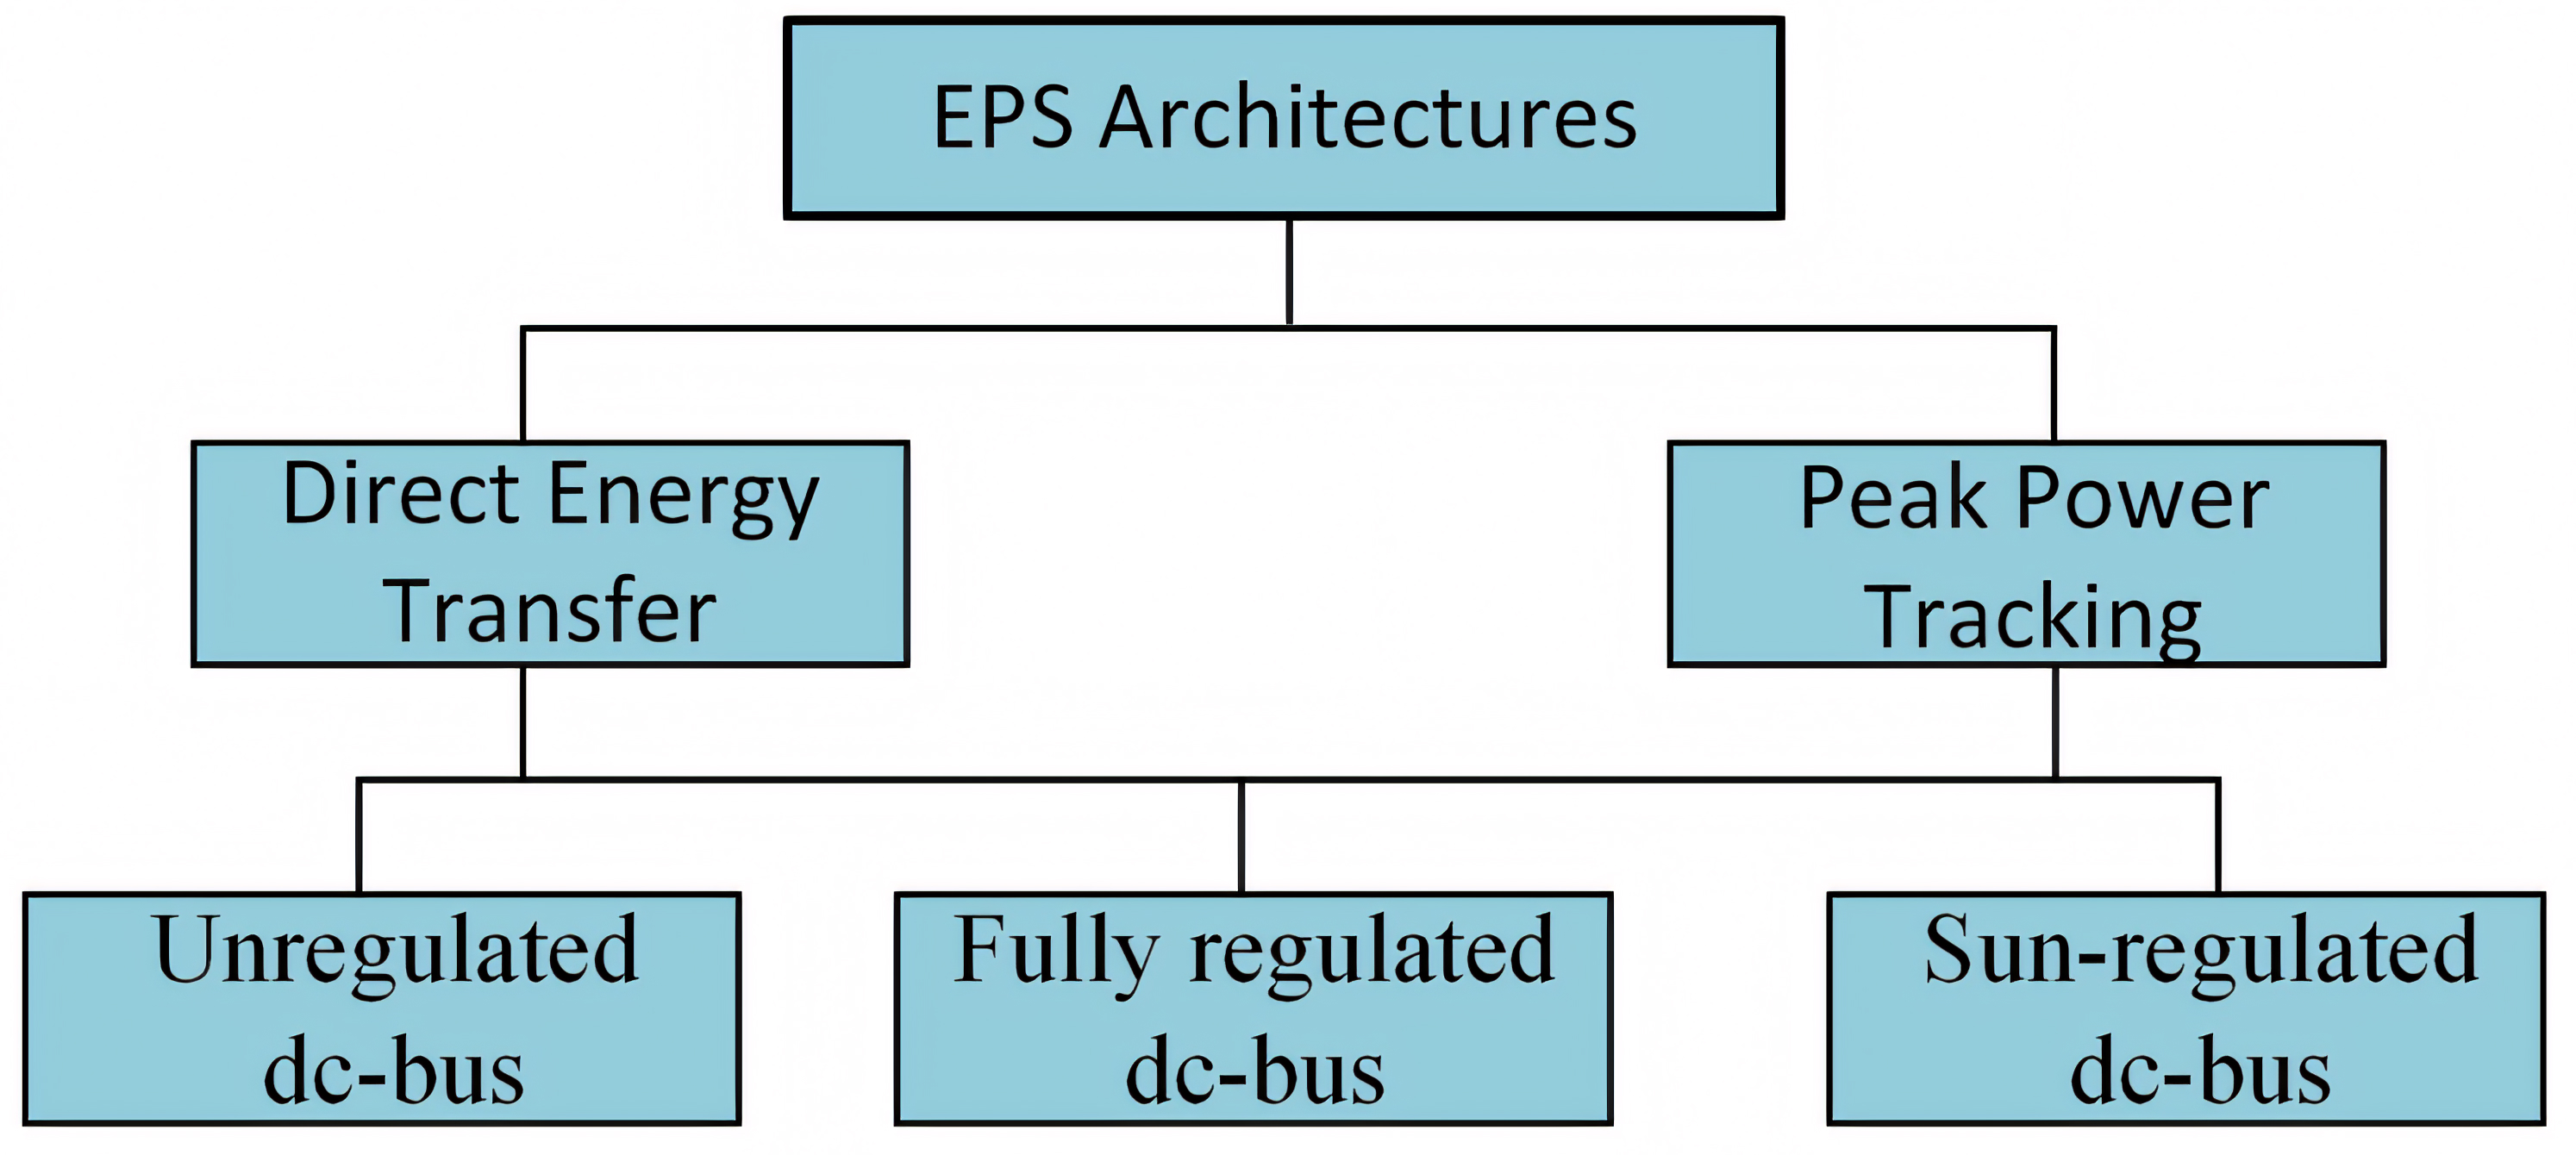
\includegraphics[width=\columnwidth]{IMGS/EPSarchitectures.jpg}
	\caption{CubeSat EPS architectures}
	\label{fig:arch}
\end{figure} 
\\ \\
Based on the interfacing of PV panels, the EPS architectures are classified as direct energy transfer (DET) and peak power tracking (PPT) architectures. 
\\ \\
In the DET architecture, the PV panels are directly connected to the battery and/or load equipment via diodes. It also uses a shunt regulator in parallel with the PV panels to absorb excess power when the battery reaches full-charge condition.
\\ \\
 In the PPT architecture, the PV panels are interfaced with a power electronic converter to extract the maximum power from the panels under widely varying operating conditions such as solar irradiation, PV panel temperature, and inclination angle. 
 \\ \\
The DET architecture requires matching of PV panel characteristics and the dc-bus voltage to generate maximum possible power which is not straightforward in the space missions. Therefore, the majority of CubeSats utilize the PPT architecture to maximize the solar energy harvest, which has limited PV panel capacity and storage capacity due to strict volume and weight constraints. 
\\ \\
The PPT architectures are further classified based on dc-bus voltage regulation: unregulated dc-bus, regulated dc-bus; and sun-regulated dc-bus. 
\\ \\
The unregulated dc-bus EPS architecture has the battery terminals directly connected to dc-bus. When the battery voltage reaches its upper limit, the MPPT converter is operated in voltage regulation mode to avoid further charging of the battery. 
\\ \\
The regulated dc-bus EPS architecture interfaces the battery with a dc–dc converter to maintain the dc-bus voltage at the predefined value. This architecture enables the operation of CubeSat at higher dc-bus voltage so that conduction and ohmic losses are reduced. 
\\ \\
In the sun regulated dc-bus EPS architecture, the dc-bus voltage is maintained at reference value only during the sunlit period. During the eclipse period, the battery gets connected to the dc-bus via a diode to supply the loads.
\\ \\

 This project focuses on the design of an EPS with a regulated DC bus and MPPT tracking.
%
%[1] shows the comparison between different CubeSat EPS architectures, from which we have identified the architecture with maximum power point tracking and a regulated DC buses to be most suitable for our application.
\\

Based on the difference between centralized and distributed architecture was discussed in [2] and we have selected centralized architecture.
\\

As discussed in [3], solar panels operate at their most efficient points with a power point tracking algorithm, allowing the extraction of maximum power from the solar panels. Hence, peak power transfer is preferred to direct power transfer.
\\

Different battery technologies used in CubeSats were discussed in [4] and Li-ion cells were selected as the energy storage device due to their high energy density and higher number of charge discharge cycles compared to LiPo and NiMH batteries.
\\

From [5], the optimum ambient temperature for charging a Lithium ion battery is +5°C to +45°C and thus, charging is limited to this range of temperature.